% \documentclass[handout]{beamer} % to ignore \pause
\documentclass[]{beamer}

%
% Choose how your presentation looks.
%
% For more themes, color themes and font themes, see:
% http://deic.uab.es/~iblanes/beamer_gallery/index_by_theme.html
%
\usetheme{default}      % or try Darmstadt, Madrid, Warsaw, ...
\usecolortheme{default} % or try albatross, beaver, crane, ...
\usefonttheme{default}  % or try serif, structurebold, ...
\setbeamertemplate{navigation symbols}{}
\setbeamertemplate{caption}[numbered]
% Frame numbers
\setbeamercolor{footline}{fg=gray}
\setbeamertemplate{footline}[frame number]
%  Take care of uncovered text
\setbeamercovered{invisible}

\usepackage[english]{babel}
\usepackage[utf8]{inputenc}
\usepackage[T1]{fontenc}
\usepackage{amsthm}
\usepackage{csquotes}
\usepackage{verbatim}

% Change \emph behaviour
\DeclareTextFontCommand{\emph}{\color{red}\em}
\newcommand{\todo}{{\large \color{red} TODO \ }}

\title[]{Problem 7: Coherence\\Problem 11: Intermediate Concepts}
\author{Katarzyna Frackowski, Falko Hemstra}
\institute{}
\date{\today}

\begin{document}
% Do not count title slide
\addtocounter{framenumber}{-1}
\begin{frame}[plain]
  \titlepage
\end{frame}

% Uncomment these lines for an automatically generated outline.
%\begin{frame}{Outline}
%  \tableofcontents
%\end{frame}

\begin{frame}{Coherence: Intuition}
    \begin{minipage}{.65\textwidth}
        \begin{itemize}
            \item Normative systems: Collection of norms
            \item Formal norm: Conditional statement
            \item Example: Given a situation, a law book tells you how to act correctly.
            % you are a guest -> be polite
            \item Question: How can we determine if our rules make sense?
        \end{itemize}
    \end{minipage}\hspace{.5cm}%
    \begin{minipage}{.3\textwidth}
        \begin{center}
            
\includegraphics[width=\textwidth]{images/law_book.jpg}
        \end{center}
    \end{minipage}%
    % Tell: No summary at the end, so listen carefully
\end{frame}

\begin{frame}{Coherence: Formalization}
    \begin{definition}[Normative System]
        A \emph{normative System} $G$ is a set of norms.
    \end{definition}
    \begin{definition}[Norm]
        A \emph{norm} $n = (c,s)$ consists of two PL formulas, a \emph{condition} $c$ and a \emph{statement} $s$. It is fulfilled if either the condition is not satisfied or the statement holds.
    \end{definition}
    \pause
    \begin{itemize}
        \item Example: \enquote{If you are a guest, be polite.}
    \end{itemize}
\end{frame}

\begin{frame}{I/O-Logic}
    \begin{itemize}
        \item Idea: Observe what, given a situation $A$, the system $G$ suggests!
        \item Formalization: Check properties of $\mathit{out}(G,A)$.
        \pause
        \item Example:
        \[A = \{..., \mathit{guest},...\},\quad G = \{...,(\mathit{guest},\mathit{polite}),...\}\]
        \[\mathit{out}(G,A) = \{...,\mathit{polite},...\}\]
        \vspace*{-\baselineskip}\pause
        \item \small Note: A set of boolean variables can be termed \emph{consistent}. For normative systems we use \emph{coherence}, since norms do not hold truth values.
    \end{itemize}
\end{frame}

\begin{frame}{Coherence: Possible Solutions (1/3)}
    \begin{itemize}
        \item Question: When is a system coherent?
    \end{itemize}
    \pause
    \begin{quote}
        $(1)$ \ $G$ is coherent \quad iff \quad $\bot \not\in \mathit{out}(G,A)$
    \end{quote}
    \pause
    \begin{itemize}
        \item Problem: Unclear which situations $A$ to examine.
    \end{itemize}
    \pause
    \begin{quote}
        $(1a)$ \ $G$ is coherent \quad iff \quad $\exists A\colon \bot \not\in \mathit{out}(G,A)$
    \end{quote}
    \pause
    \begin{itemize}
        \item This definition seems too weak.
        \item Consider $G=\{(c,s),(c,\neg s)\}$. Since $\bot \not\in \mathit{out}(G,\emptyset)$, the system is coherent.
    \end{itemize}
\end{frame}

\begin{frame}{Coherence: Possible Solutions (2/3)}
    \begin{itemize}
        \item The dual of $(1a)$ is:
    \end{itemize}
    \begin{quote}
        $(1b)$ \ $G$ is coherent \quad iff \quad $\forall A \colon \bot \not\in \mathit{out}(G,A)$
    \end{quote}
    \begin{itemize}
        \item This seems too strong.
        \pause
        \item Idea: Consider only foreseeable situations!
    \end{itemize}
    \begin{quote}
        $(1c)$ \ $G$ is coherent \quad iff \quad $\forall (c,s) \in G  \colon \bot \not\in \mathit{out}(G,c)$
    \end{quote}
    \pause
    \begin{itemize}
        \item This requires too many norms to function.
        \item Let $(c_1,s_1)$ and $(c_2,s_2)$ be norms, then $c_1 \land c_2$ is not a situation we consider for coherence with $(1c)$.
        % Example: (guest, polite), (attacked, not polite)
        % Explain: (1d) fixes this problem, but there still is $(a,\neg a)$
    \end{itemize}
\end{frame}

\begin{frame}{Coherence: Possible Solutions (3/3)}
    \begin{itemize}
        \item Question: The norm $(c,\neg c)$ creates a conflict between input and output. Should this norm be allowed?
    \end{itemize}
    \pause
    \begin{quote}
        $(2)$ \ $G$ is coherent \quad iff \quad $\mathit{out}(G,A) \cup A \not\models \bot$
    \end{quote}
    \pause
    \begin{itemize}
        \item With (2), norm violation causes incoherence.
        \item Example: An impolite guest
        \[(\mathit{guest}, \mathit{polite})\in G, \quad \mathit{guest}, \neg\mathit{polite} \in A\]
        \[\mathit{out}(G,A) \cup A = \{...,\mathit{polite},\neg\mathit{polite},...\} \models \bot\]
    \end{itemize}
\end{frame}

\begin{frame}{Coherence: Output under constraints}
    \begin{itemize}
        \item Idea: To determine coherence we examine systems in specific situations and under certain constraints.
    \end{itemize}
    \begin{definition}[Output under constraints]
        Let $G$ be a normative system and $A$ and $C$ two sets of propositional formulas. Then $G$ is \emph{coherent} in $A$ under constraints $C$ iff $\mathit{out}(G,A) \cup C$ is consistent.
    \end{definition}
\end{frame}

\begin{frame}{Coherence: Caveats}
    \begin{itemize}
        \item Consider the norm $(\mathit{broken},\neg \mathit{broken})$ which commands agents to fix things they find to be broken. Is this a reasonable norm?
        \pause
        \item Problem: Fixing takes time
        \[\mathit{out}(G,A) \cup A = \{\neg \mathit{broken}\} \cup \{\mathit{broken}\} \models \bot\]
        \vspace*{-\baselineskip}\pause %  use this to remove weird empty pace introduced by \pause
        \item Implication: The presented approach is \emph{static}!
        \item We \emph{can not} instruct agents on how to act.
        \item We \emph{can} describe properties of still frames.
    \end{itemize}
\end{frame}

\begin{frame}
    \centering\LARGE
    Problem 11:\par
    Meaning Postulates and Intermediate Concepts
\end{frame}

\begin{frame}{Introduction}
    \begin{definition}[Meaning Postulates]
    Stipulative definition, legal meaning.
    \end{definition}

    \begin{definition}[Intermediate Concepts]
    Relation between legal definitions and words describing natural facts.
    \end{definition}
\end{frame}

\begin{frame}{Example - A Verdict}      
    \begin{quote}
        An act of theft is punished by a prison sentence not exceeding 5 years or a fine.
    \end{quote}
\end{frame}

\begin{frame}{Example - A Verdict}      
    \begin{quote}
        An act of \emph{theft} is punished by a prison sentence not exceeding 5 years or a fine.
    \end{quote}
\end{frame}

\begin{frame}{Example - A Definition} 
    \begin{quote}
        Someone commits an act of theft if that person has taken a movable object from the possession of another person into his own possession with the intention to own it, and if the act occurred without the consent of the other person or some other legal authorization.
    \end{quote}
 \hspace{1cm}
 
     $\rightarrow$ \textcolor{blue}{meaning postulate for the word \emph{theft}}
\end{frame}

\begin{frame}{Example - A Definition}
    \begin{quote}
        Someone commits an act of theft if that \textcolor{blue}{person} has taken a \textcolor{blue}{movable object} from the possession of another person into his own \textcolor{blue}{possession} with the intention to \textcolor{blue}{own} it, and if the act occurred without the consent of the other person or some other legal authorization.
    \end{quote}
\vspace{1cm}
    \begin{quote}
        A \textcolor{blue}{person} in the sense of the law is a \emph{human being} that has been \emph{born}.
    \end{quote}
    
\vspace{1cm}
\hspace{1cm}
    $\rightarrow$ \textcolor{blue}{meaning postulates and \emph{intermediate concepts}}
\end{frame}

\begin{frame}{Possible Solution 1: Relational Expressions}      
    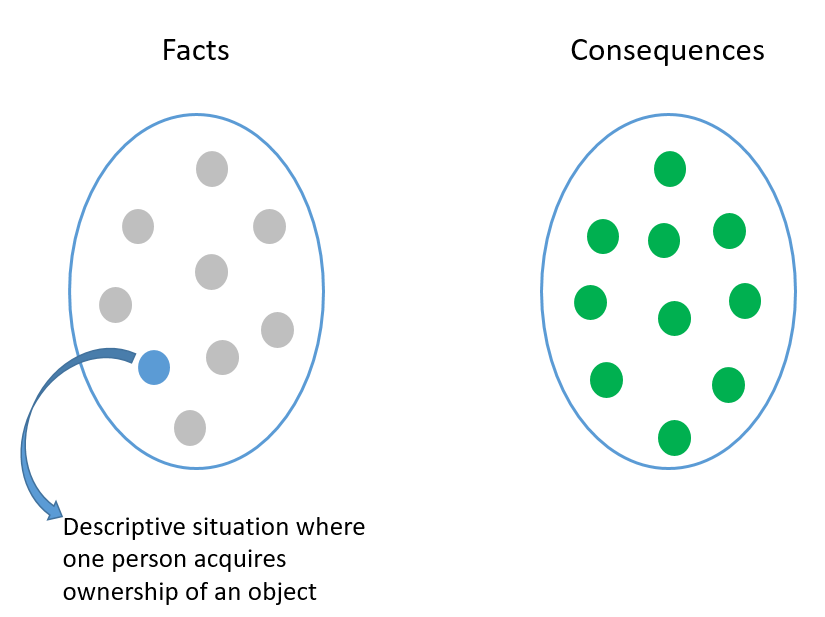
\includegraphics[width=10cm]{images/Sem_Pres_11_1.png}
\end{frame}

\begin{frame}{Possible Solution 1: Relational Expressions}      
    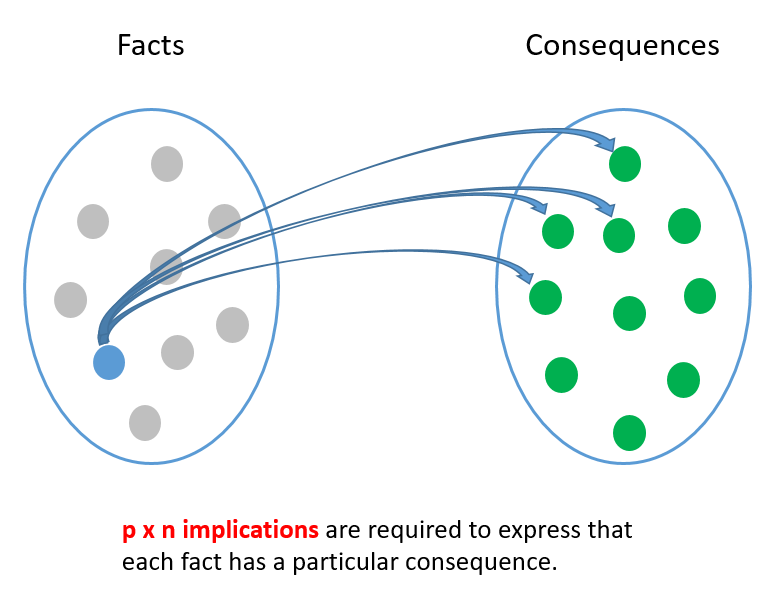
\includegraphics[width=10cm]{images/Sem_Pres_11_2.png}
\end{frame}

\begin{frame}{Possible Solution 1: Relational Expressions}      
    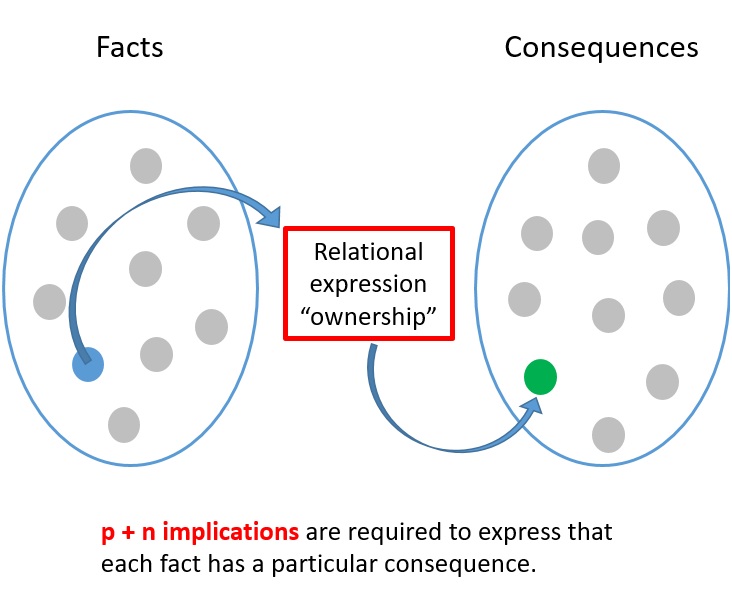
\includegraphics[width=10cm]{images/Sem_Pres_11_3.png}
\end{frame}

\begin{comment} % stattdessen Grafiken erstellen zum einfacheren Verständnis
\begin{frame}{Possible Solution 1: Relational Expressions}
    \begin{itemize}
        \item introduce relational terms between acts and consequences
        \item example:
        \begin{itemize}
            \item $F_n$: descriptive situation where one person acquires ownership of an object
            \item $C_n$: legal consequences of this ownership
            \item $p x n$ implications to express that a fact $F_i$ has a consequence $C_j$
            \item introduction of relational term \enquote{ownership}
            \item reduces implications to $p + n$
        \end{itemize}
    \end{itemize}
\end{frame}
\end{comment}


\begin{frame}{Possible Solution 2: I/O-Logic}
    \begin{itemize}
        \item enhance I/O logic with separate set of intermediates
        \item employ a \emph{separate set T of intermediates $(a,x)$} with
        \begin{itemize}
            \item $a =$ facts
            \item $x =$ obtaining legal term
            \item $G =$ set of norms
        \end{itemize}
        \item use $A \cup out(T,A)$ as input to derive an output along G
    \end{itemize}
\end{frame}

\begin{frame}{Possible Solution 2: I/O-Logic}
    \begin{itemize}
        \item Example: I/O Logic
        \[A = \{..., \mathit{dog},...\},\quad G = \{...,(\mathit{\neg{dog}},\mathit{premises}),...\}\]
        \[\mathit{out}(G,A) = \{...,\textit{no-dogs-on-premises},...\}\]
        \pause
        \item Example: I/O Logic with intermediate concept T
        \[A = \{..., \mathit{dog},...\},\quad G = \{...,(\mathit{\neg{dog}},\mathit{premises}),...\}\]
        \[T = \{...,(\textit{blind-person, guide-dogs}),...\}\]
        \[\mathit{out}(T,A) \, \cup \, A = \{...,\textit{no-dogs-on-premises, except-blind-people},...\}\]
    \end{itemize}
\end{frame}

\begin{frame}{Critique}
    \begin{itemize}
        \item Length
        \item Lack of analysis, abstraction and formalization
    \end{itemize}
\end{frame}

\end{document}
